\documentclass[a4paper,11pt]{article}
\usepackage[francais]{babel}
%% Prévu pour compiler avec lualatex
% \usepackage[utf8]{inputenc}
 \usepackage{fontspec}
\usepackage{libertine}
% \usepackage[T1]{fontenc}
\usepackage{graphicx}
\usepackage{fancyhdr}
\usepackage[top=2.5cm, bottom=2.5cm, left=2cm, right=2cm]{geometry}
\usepackage{listings}
\usepackage[utf8]{luainputenc}
\usepackage[hidelinks]{hyperref}
\usepackage{caption}

\lfoot{\bsc{Enseirb-Matmeca}}
\rfoot{Informatique --- 3\ieme{} année}

\pagestyle{fancy}
\begin{document}

\begin{titlepage}
  \begin{center}

    \begin{center}
      
\includegraphics[width=4cm]{EM.jpg}
    \end{center}

    \vspace*{1cm}
        
    \rule{0.75\linewidth}{0.7mm}\\[0.4cm]
    {\Huge Rapport TP2 --- MPI\\[0.4cm]}
    \rule{0.75\linewidth}{0.7mm} \\[1.5cm]

    {\Large Bazire \bsc{Houssin}\\Sylvain \bsc{Vaglica}\\Stéphane \bsc{Castelli}\\[2cm]}
    {\Large Mardi 5 Novembre 2013}
  \end{center}
\end{titlepage}

\tableofcontents
\clearpage
\section{Introduction}


Le but de ce projet est de simuler les interactions gravitationnelles entre des corps placés dans un espace sans frottement, notamment des corps de grande masse tels que les corps célestes. Lorsque ce nombre de corps est élevé, la puissance de calcul nécessaire pour déterminer toutes les attractions est importante, car chaque corps dans une certaine mesure influe sur tous les autres. Le point positif, c'est qu'il est trivial de paralléliser les calculs car ceux-ci sont tous indépendants. MPI est donc un moyen efficace pour réduire la durée d'exécution sur une machine parallèle.

La force de gravitation s'applique à l'infini dans toute les directions, selon la formule

\[
\| \vec{F}_{A\rightarrow B} \| = G \cdot \frac{M_A \cdot M_B}{\mathit{AB^3}} \cdot \mathit{\vec{AB}}
\]

Pour les tests, nous nous sommes inspirés du système solaire.

\section{Présentation de l'algorithme}
L'algorithme de calcul séquentiel pour calcul de forces gravitationnelle sur un système de $n$ masses distinctes, consiste à répéter pour chaque masse $m$ les étapes suivantes:

\begin{itemize}
\item Pour chaque masse $m'$ distincte de $m$, calculer la force d'interaction gravitationnelle entre les deux masses.
\item Calculer la force résultante (direction et norme) de toutes les autres masses sur $m$.
\item Trouver la distance minimale entre n'importe quelle paire des masses.
\item Calculer l'accélération résultante de la masse $m$.
\item En déduire sa vitesse, le pas de calcul ($dt$) et sa nouvelle position.
\end{itemize}

Les formules utilisées pour l'accélération, la vitesse et de la position sont celles obtenues par l'application du principe fondamental de la dynamique sur chacune des masses.


Pour la version distribuée,% stribuée
le stockage de l'ensemble des masses est réparti en nombre égal sur l'ensemble des processus. Chaque processus effectue les calculs sur les masses qu'il possède en local, mais doit régulièrement envoyer les données aux autres processus. La topologie et les communications seront décrites dans la partie suivante. On obtient donc l'algorithme suivant, à appliquer sur chaque masse $m$ locale :

\begin{itemize}
\item On déterminer tout d'abord le pas de calcul (commun à tout les processus), grâce à la distance minimale entre tous les couples de masses mémorisée à l'itération précédente.
\item Pour chaque masse  reçue $m'$ distincte de $m$, calculer la force d'interaction gravitationnelle entre les deux masses.
\item Calculer l'accélération de la masse $m$, induite par $m'$.
\item En déduire sa vitesse et sa nouvelle position induite par $m'$.
\end{itemize}


Pour chacun des deux algorithmes, on peut itérer indéfiniment afin d'obtenir une trajectoire de chacune des masses plus ou moins longues. Dans les deux cas, on effectue un premier tour de boucle sans modifier les positions afin de déterminer le pas de calcul qui est donné par la formule :

\[
\sqrt{\|\vec{v}\|^2 + 0.02 \times \|\vec{a}\| \times \mathit{D_{min}}} - \frac{\| \vec{v}\|}{\| \vec{a} \|}
\] 
Où $\vec{a}$ est l'accélération du point, $\vec{v}$ sa vitesse, et $\mathit{D_{min}}$ la distance minimale avec les autres points.




\section{Topologie, répartition des données et communications}

Comme expliqué dans la partie précédente, chaque processus possède une partie des données en local, et doit régulièrement recevoir la nouvelle position de chacune des masses. On choisit donc une structure en anneau, chaque processus stocke le poids, la position, la vitesse et l'accélération de ses masses. De plus, chaque processus utilise deux buffers temporaires, l'un lui permettant de recevoir les données pendant que les calculs sont effectués sur le premier jeu de données. Cela permet de recouvrir les communication par les calculs. Ainsi, pour un pas de calcul (une itération de l'algorithme, permettant de calculer le nouvel état du système après un instant $dt$) et $p$ processus, on effectue $p$ fois les étapes suivantes:
\begin{itemize}
\item Chaque processus reçoit les données de son prédécesseur dans l'anneau et les stocke dans le premier buffer, et envoie les données présentes dans le deuxième buffer à son successeur. Si $p = 0$, on copie au préalable les données locales dans le buffer 2 avant de l'envoie.
\item Pendant ce temps, chaque processeur calcule l'influence de chacune des masses du deuxième buffer, sur chacune des masses qu'il stocke en local (les masses doivent être distinctes).
\end{itemize}
 A chaque itération, on inverse les buffers 1 et 2, l'un devenant celui de réception, l'autre celui contenant les données devant être traitées.

Comme expliqué dans la partie précédente, chaque processus possède une partie des données en local, et doit régulièrement recevoir la nouvelle position de chacune des masses. On choisit donc une structure en anneau, chaque processus stocke le poids, la position, la vitesse et l'accélération de ses masses. De plus, chaque processus utilise deux buffers temporaires, l'un lui permettant de recevoir les données pendant que les calculs sont effectués sur le premier jeu de données. Cela permet de recouvrir les communications par les calculs. Ainsi, pour un pas de calcul (une itération de l'algorithme, permettant de calculer le nouvel état du système après un instant $dt$) et $p$ processus, on effectue $p$ fois les étapes suivantes:

\begin{itemize}
\item Chaque processus reçoit les données de son prédécesseur dans l'anneau et les stocke dans le premier buffer, et envoie les données présentes dans le deuxième buffer à son successeur. Si $p = 0$, on copie au préalable les données locales dans le buffer 2 avant de l'envoie.
\item Pendant ce temps, chaque processeur calcule l'influence de chacune des masses du deuxième buffer, sur chacune des masses qu'il stocke en local (les masses doivent être distinctes).
\end{itemize}
 A chaque itération, les buffers 1 et 2 sont inversés, l'un devenant celui de réception, l'autre celui contenant les données devant être traitées.

  A la fin des $p$ rotations, les données initiales sont revenues en positions initiale (elles ont parcouru l'ensemble des noeuds de l'anneau), et l'influence de toutes les masses sur chacune des données locales a donc été calculée.
 On peut donc commencer une nouvelle itération de l'algorithme pour calculer le nouvel état du système. en commençant par calculer le pas de calcul $dt$, en fonction de la distance minimale entre deux masses quelconques, distance mémorisée lors de l'itération précédente.
 
 

\section{Vérifications et Performances}
\subsection{Vérifications}
Afin de vérifier la correction de notre programme, nous l'avons testé sur différents exemples d'abord simple (deux objets immobiles, de masses identiques ou différentes), avant de passer à des exemples plus complexes.
L'exemple suivant est une simulation de la rotation de la Terre autour du Soleil (en (0,0)).
\begin{figure}[h!]
  \centering
  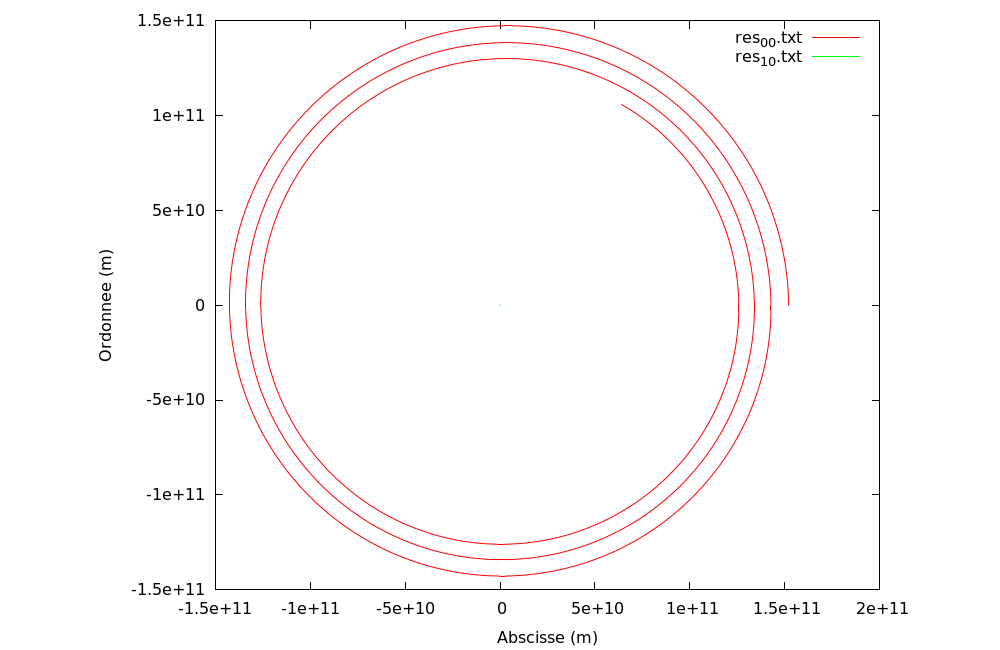
\includegraphics[width=\textwidth]{orbite_terre.png}
  \caption{Performance du programme}
  \label{perf}
\end{figure}Comme il est possible de le constater, l'orbite est sur notre image une spirale, augurant un sombre futur pour notre planète. Cette incohérence est du à l'imprécision des données initiales utilisées, et possiblement aussi à la taille du pas des itérations.
Cependant, la trajectoire est logique et régulière, bien que non cohérente avec la réalité. Elle reste correcte par rapport au modèle physique.

Il en est de même pour le graphe suivant, représentant les cinq premières planètes du système solaire (Mercure, Vénus, Terre, Mars, Jupiter) ainsi que le Soleil (en 0,0).
\begin{figure}[h!]
  \centering
  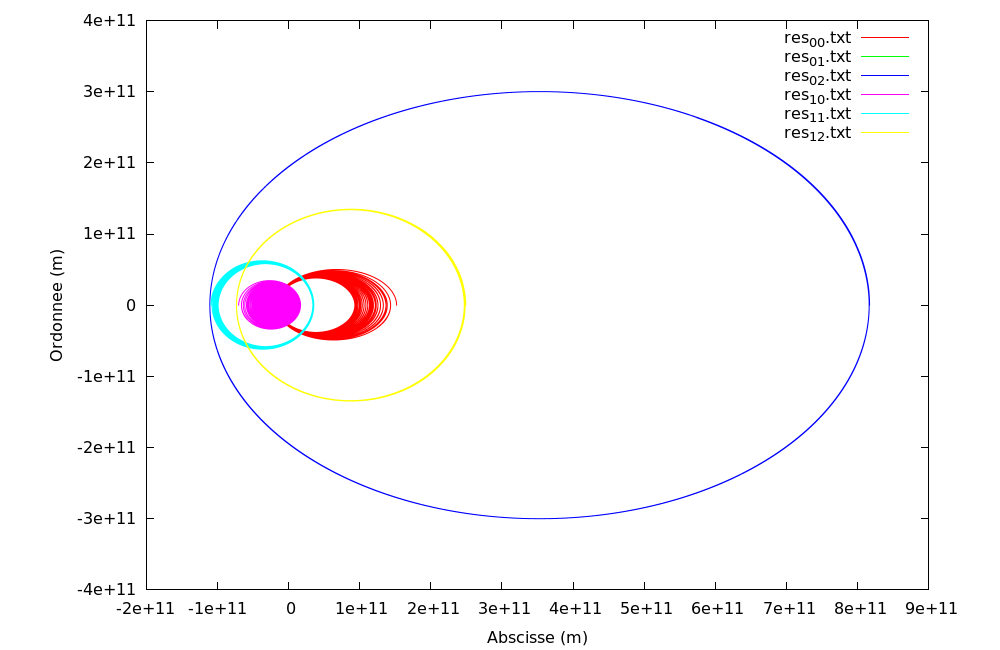
\includegraphics[width=\textwidth]{systeme.png}
  \caption{Performance du programme}
  \label{perf}
\end{figure}
Les trajectoires restent plausibles, même si complètement différentes de la réalité.  
\subsection{Performances}
Ci-dessous un graphique illustrant le temps d'exécution du programme sur un grand nombre de points, effectué sur une machine doté de 48 coeurs. 
Les points sont répartis de manière à ne pas être à la même position, et dotés d'une masse très faible, garantissant que les calculs se déroulent correctement (pas de division par zéro ou autres opérations interdites), et en ne bougeant que très peu (pas de risque de collision, et donc de calculs faux). 

%INSERT GRAPHIQUE HERE

Comme attendu, les performances pour 48 processus sont largement meilleurs, et décroissent alors que le nombre de processus diminue.
Les performances pour un nombre de points faibles sont relativement proches, peu importe le nombre de processus, désignant les parties séquentielles et systèmes non réductibles de notre programme.

Pour le cas avec 6400 objets, le speed up entre l'exécution sur 48 processus et 1 seul est de 9,45 (de 474 secondes, le temps réel devient à 50,25).
Le speed up est important, et pourrait sans doute l'être encore plus si les données fournies pour chaque processus étaient encore plus importantes (ici, 133-134 données par objet).
Il est possible que ce nombre ne soit pas suffisant pour couvrir entièrement les calculs.

\section{Conclusion}

La puissance de MPI se ressent pleinement lorsque l'on a des calculs lourds sans dépendances entre eux. Exécuté en séquentiel, sur un grand nombre de planètes, cela prendrait un temps considérable. Grâce au passage en parallèle, pour distribuer à la fois les données et le travail entre un nombre quelconque de processus, on arrive à diminuer fortement le temps d'exécution. De plus, une bonne répartition des données entre les processus permet de mettre en place un recouvrement des communications entre les processus par les calculs. Malgré ça, si on augmente fortement le nombre de processus sans augmenter le nombre de données, on se retrouve rapidement dans le cas où les calculs ne suffisent plus à recouvrir le temps des communications. L'idéal est donc de garder un équilibre entre le nombre de processus et la quantité de données par processus.

\end{document}
